\documentclass[reqno]{amsart}
\usepackage[utf8]{inputenc}
\usepackage[margin=1in]{geometry}
\usepackage[usenames, dvipsnames]{xcolor}
\usepackage{graphicx}
\usepackage{mathtools}
\usepackage{amssymb}
\usepackage{amsthm}
\usepackage{fancyhdr}
\usepackage{adforn}
\usepackage{xparse}
\usepackage{tikz}
\usetikzlibrary{fadings}
%\usetikzlibrary{matrix, positioning, calc}
% Additional math macros that I want in both my notes and my psets
\usepackage[sc, noBBpl]{mathpazo}
\usepackage{mathrsfs}
\usepackage[T1]{fontenc}
\usepackage{calligra}
\usepackage{microtype}
\usepackage[all]{xy}
\usepackage{slashed}
\newcommand{\A}{\mathbb A}
\newcommand{\cat}{\mathsf}
\newcommand{\sC}{\cat C}
\newcommand{\sD}{\cat D}
\newcommand{\sS}{\cat S}
\newcommand{\sA}{\mathscr A}
\newcommand{\sF}{\mathscr F}
\newcommand{\sG}{\mathscr G}
\renewcommand{\P}{\mathbb P}
\newcommand{\cO}{\mathscr O}
\newcommand{\sI}{\mathscr I}
\DeclareMathOperator{\coker}{coker}
\renewcommand{\Im}{\operatorname{Im}}
\newcommand{\pt}{\mathrm{pt}}
\DeclareMathOperator{\Hom}{Hom}
\newcommand{\op}{^{\mathsf{op}}}
\newcommand{\Id}{\mathrm{Id}}
\DeclareMathOperator{\Mat}{Mat}
\newcommand{\m}{\mathfrak m}
%\newcommand{\p}{\mathfrak p}
\newcommand{\q}{\mathfrak q}
\DeclareMathOperator{\MSpec}{MSpec}
\DeclareMathOperator{\Spec}{Spec}
\newcommand{\Top}{\cat{Top}}
\newcommand{\Ring}{\cat{Ring}}
\newcommand{\Mod}{\cat{Mod}}
\DeclareMathOperator{\res}{res}
\newcommand{\Alg}{\cat{Alg}}
\newcommand{\Fun}{\cat{Fun}}
\newcommand{\AffSch}{\cat{AffSch}}
\newcommand{\Ab}{\cat{Ab}}
\DeclareMathOperator{\bl}{--}
\DeclareMathOperator{\Free}{Free}
\DeclareMathOperator{\For}{For}
\newcommand{\Set}{\cat{Set}}
\newcommand{\LocRing}{\cat{LocRing}}
\newcommand{\Grp}{\cat{Grp}}
\newcommand{\Sch}{\cat{Sch}}
\newcommand{\inHom}{\operatorname{\underline{\Hom}}}
\DeclareMathOperator{\Frac}{Frac}
\DeclareMathOperator{\Gal}{Gal}
\DeclareMathOperator{\Nil}{Nil}
\newcommand{\pre}{\sC^{\text{pre}}}
\newcommand{\sh}{_{\text{sh}}}
\newcommand{\G}{\mathbb G}
\DeclareMathOperator{\Proj}{Proj}
\newcommand{\sM}{\mathscr M}
\newcommand{\sV}{\mathscr V}
\newcommand{\fU}{\mathfrak U}
\newcommand{\GL}{\mathrm{GL}}
\DeclareMathOperator{\Sym}{Sym}
% http://tex.stackexchange.com/questions/141434/how-to-type-sheaf-hom
\DeclareMathOperator{\shom}{\mathscr{H}\text{\kern -4pt {\calligra\large om}}\,}
\newcommand{\sL}{\mathscr L}
\DeclareMathOperator{\QC}{QC}
\DeclareMathOperator{\Supp}{Supp}
\newcommand{\sN}{\mathscr N}
\DeclareMathOperator{\Ann}{Ann}
\DeclareMathOperator{\Der}{Der}
\newcommand{\ctcpx}[1]{(#1)^{\text{der}}}
\newcommand{\Dist}{\mathsf{Dist}}
\newcommand{\shdi}{\operatorname{Sh}_{\Dist}}
\DeclareMathOperator{\Sh}{Sh}
\newcommand{\shz}{\mathsf{Sh}_{\text{\rm Zar}}}
\DeclareMathOperator{\Gr}{Gr}
% Source: http://tug.org/pipermail/xy-pic/2001-July/000015.html
\newcommand{\pullbackcorner}[1][dr]{\save*!/#1+1.2pc/#1:(1,-1)@^{|-}\restore}
\newcommand{\pushoutcorner}[1][dr]{\save*!/#1-1.2pc/#1:(-1,1)@^{|-}\restore}
\newcommand{\TDel}{\mathrm{2\Delta}}
\DeclareMathOperator{\Bl}{B\ell}
\newcommand{\cR}{\mathcal R}
\newcommand{\cL}{\mathcal L}
\newcommand{\cH}{\mathcal H}
\newcommand{\refR}{\reflectbox{\(\cR\)}}

\renewcommand{\a}{\alpha}
\renewcommand{\b}{\beta}
%\newcommand{\e}{\epsilon}
\renewcommand{\l}{\lambda}
\renewcommand{\L}{\Lambda}
\newcommand{\g}{\gamma}
\newcommand{\s}{\sigma}
\newcommand{\z}{\zeta}
\newcommand{\RR}{\mathbb{R}}
\newcommand{\NN}{\mathbb{N}}
\newcommand{\QQ}{\mathbb{Q}}
\newcommand{\ZZ}{\mathbb{Z}}
\newcommand{\CC}{\mathbb{C}}
\newcommand{\cC}{\mathcal{C}}
\newcommand{\f}{\frac}
\newcommand{\p}{\partial}
\renewcommand{\P}[3][]{\f{\partial^{#1} #2}{\partial #3 ^{#1}}}
%\newcommand{\avg}[1]{\langle #1 \rangle}
\newcommand{\avg}[1]{\left< #1 \right>}
\newcommand{\?}{\overset{?}{=}}
\newcommand{\Int}{\int_{-\infty}^\infty}
\newcommand{\ket}[1]{\left| #1 \right>} % for Dirac bras
\newcommand{\bra}[1]{\left< #1 \right|} % for Dirac kets
\newcommand{\braket}[2]{\left< #1 \vphantom{#2} \right|
 \left. #2 \vphantom{#1} \right>} % for Dirac brackets
\newcommand{\pv}{\vec{p}}

\newcommand{\grad}[1]{\gv{\nabla} #1} % for gradient
\let\divsymb=\div % rename builtin command \div to \divsymb
\renewcommand{\div}[1]{\gv{\nabla} \cdot #1} % for divergence
\newcommand{\curl}[1]{\gv{\nabla} \times #1} % for curl
\renewcommand{\labelenumi}{(\alph{enumi})}
\let\vaccent=\v % rename builtin command \v{} to \vaccent{}
\renewcommand{\v}[1]{\ensuremath{\mathbf{#1}}}
\newcommand{\uv}[1]{\ensuremath{\mathbf{\hat{#1}}}} % for unit vector
\newcommand{\gv}[1]{\ensuremath{\mbox{\boldmath$ #1 $}}} 
% for vectors of Greek letters
\usepackage{hyperref}
\usepackage{siunitx}

%\usepackage[compat=1.1.0]{tikz-feynman}

% TODO fiddle with colors
\definecolor{newblue}{HTML}{1F98A6}
\definecolor{newred}{HTML}{D95448}
\definecolor{neworange}{HTML}{F29441}
\hypersetup{
	colorlinks,
	linkcolor=newred,
	citecolor=neworange,
	urlcolor=newblue!80!black,
}
\usepackage[all]{hypcap}
\pagestyle{plain}
\setcounter{tocdepth}{1}


\usepackage{titlesec}
\titleformat{\section}[frame]
  {\normalfont}
  {\filright
   \footnotesize
   \enspace Lecture \arabic{section}.\enspace}
  {8pt}
  {\Large\bfseries\filcenter}
\usepackage[dotinlabels]{titletoc}
\titlecontents{section}[1.5em]{}{\contentslabel{2.3em}}{\hspace*{-2.3em}}{\hfill\contentspage}

\renewcommand{\sectionmark}[1]{\markleft\thesection. #1}

\fancyhf{}
\fancyhead[RO,LE]{\small\thepage}
\fancyhead[LO]{\small\slshape\nouppercase{\rightmark}}
\fancyhead[RE]{\small\slshape Advanced Quantum Field Theory Lecture Notes}
\setlength{\headheight}{11.0pt}
\pagestyle{fancy}

\numberwithin{equation}{section}
\newcommand{\orbreak}{
\begin{center}
	\adforn{17}\;\(\cdot\)\;\adforn{18}
	\vspace{0.2cm}
\end{center}
}

\renewcommand{\labelitemi}{\(\circ\)}

% I wanted to allow one to reference parts of a thm/cor/etc. and have it print the thm number too, e.g. 29.2(1),
% but this isn't working right now. Probably the best way to do this would be to play around with enumitem to
% define a new enumerate-like counter and then just use that directly instead of enumerate in comp.

% This feels really wobbly, but so far it's working
\NewDocumentEnvironment{comp}{mm}{%
	\csname #1\endcsname\hfill
	\csname #2\endcsname
}{
	\csname end#2\endcsname
	\csname end#1\endcsname
}

% usage:
% \shortexact[f][g]{A}{B}{C},
%
%			 f    g
% for 0 -> A -> B -> C -> 0,
\DeclareDocumentCommand{\shortexact}{O{} O{} mmmm}{
\xymatrix{
	0\ar[r] & #3\ar[r]^-{#1} & #4\ar[r]^-{#2} & #5\ar[r] & 0#6
}}
% exactly the same, but for 0 -> A -> B -> C
\DeclareDocumentCommand{\leftexact}{O{} O{} mmmm}{
\xymatrix{
	0\ar[r] & #3\ar[r]^-{#1} & #4\ar[r]^-{#2} & #5 #6
}}
% ... and the same, for A -> B -> C -> 0
\DeclareDocumentCommand{\rightexact}{O{} O{} mmmm}{
\xymatrix{
	#3\ar[r]^-{#1} & #4\ar[r]^-{#2} & #5\ar[r] & 0#6
}}



% usage:
% X\dblarrow[r] & Y
%   f
% X => Y
%   g
\DeclareDocumentCommand{\dblarrow}{O{} O{} O{}}{
	\ar@<0.4ex>[#1]^-{#2}\ar@<-0.4ex>[#1]_-{#3}
}
% Note: it would be a useful exercise to figure out how to define this so it can be used as
% \dblarrow[r]^f_g

\everyentry={\displaystyle}

\newcommand{\N}{\mathbb N}
\newcommand{\Z}{\mathbb Z}
\newcommand{\Q}{\mathbb Q}
\newcommand{\R}{\mathbb R}
\newcommand{\C}{\mathbb C}
\newcommand{\F}{\mathbb F}
\newcommand{\vp}{\varphi}
\newcommand{\term}{\emph}
\renewcommand{\vec}[1]{\boldsymbol{\mathbf{#1}}}
\DeclarePairedDelimiter\paren{(}{)}
%\DeclarePairedDelimiter\ang{\langle}{\rangle}
\DeclarePairedDelimiter\abs{\lvert}{\rvert}
\DeclarePairedDelimiter\norm{\lVert}{\rVert}
\DeclarePairedDelimiter\bkt{[}{]}
\DeclarePairedDelimiter\set{\{}{\}}
% Swap paren* and paren, etc., so that the normal version resizes by default.
% Meanwhile, one can use \paren*[\Big]{...} to customize the size easily.
% It would be interesting to wrap this up into a custom \definedelimiter command...
\makeatletter
	\let\oldparen\paren
	\def\paren{\@ifstar{\oldparen}{\oldparen*}}
	\let\oldbkt\bkt
	\def\bkt{\@ifstar{\oldbkt}{\oldbkt*}}
\makeatother
\newcommand{\e}{\varepsilon}
\def\qedsymbol{{\small{\ensuremath{\boxtimes}}}}
\newcommand{\inj}{\hookrightarrow}
\newcommand{\surj}{\twoheadrightarrow}
\DeclareMathOperator{\id}{id}
\newcommand{\ud}{\,\mathrm{d}}
\renewcommand{\d}{\mathrm d}
\newcommand{\dfr}[2]{\frac{\mathrm d #1}{\mathrm d #2}}
\newcommand{\pfr}[2]{\frac{\partial #1}{\partial #2}}

%\catcode`\"=13
%\newcommand{"}[1]{^{(#1)}}
\newtheorem{thm}[equation]{Theorem}
\newtheorem*{thm*}{Theorem}
\newtheorem{lem}[equation]{Lemma}
\newtheorem*{lem*}{Lemma}
\newtheorem{cor}[equation]{Corollary}
\newtheorem{prop}[equation]{Proposition}
\newtheorem{obs}[equation]{Observation}
\theoremstyle{definition}
\newtheorem{ex}[equation]{Exercise}
\newtheorem{exm}[equation]{Example}
\newtheorem{defn}[equation]{Definition}
\newtheorem*{claim}{Claim}
\theoremstyle{remark}
\newtheorem*{rem}{Remark}
\newtheorem*{fct}{Fact}
\newtheorem*{note}{Note}

\begin{document}
\title{Symmetries, Fields, and Particles}
\author{Ian Lim\\ Michaelmas 2018}
\maketitle
{\small\noindent These notes were taken for the \textit{Symmetries, Fields, and Particles} course taught by Nick Dorey at the University of Cambridge as part of the Mathematical Tripos Part III in Michaelmas Term 2018. I live-\TeX ed them using Overleaf, and as such there may be typos; please send questions, comments, complaints, and corrections to 
\href{mailto:itel2@cam.ac.uk?subject=SFP\%20Lecture\%20Notes}{\texttt{itel2@cam.ac.uk}}.\\
Many thanks to Arun Debray for the {\LaTeX} template for these lecture notes: as of the time of writing, you can find him at \url{https://web.ma.utexas.edu/users/a.debray/}.}

\tableofcontents

\section{Symmetries, Fields, and Start-icles: Thursday, October 4, 2018}
	\begin{quote}\textit{$2=\pi=i=-1$ in these lectures.} --a former lecturer of Prof. Allanach's.\end{quote}
To begin with, some logistic points. The notes and much of the course material will be based on \href{http://www.damtp.cam.ac.uk/user/tong/qft/qft.pdf}{David Tong's QFT notes} plus some of Prof. Allanach's on cross-sections and decay rates. See \url{http://www.damtp.cam.ac.uk/user/examples/indexP3.html} and in particular \url{http://www.damtp.cam.ac.uk/user/examples/3P1l.pdf} for the notes on cross-sections. In revising these notes, I'll be cross-referencing the Tong QFT notes as well as my copy of Anthony Zee's \textit{Quantum Field Theory in a Nutshell,} which takes a different pedagogical order in starting from the path integral formalism and introducing second quantization (the approach described here) later. Any good education in QFT requires an understanding of both formalisms, and we'll see the path integral next term in \emph{Advanced Quantum Field Theory}.\footnote{Note that the path integral formulation from \emph{Statistical Field Theory}, also taught this term, is precisely equivalent to the path integral that appears in QFT under the identification of one of the Euclidean dimensions of a statistical field theory with the imaginary time dimension of a QFT. This will be more obvious in hindsight.}

After Tuesday's lecture, we'll be assigned one of four course tutors:
\begin{itemize}
    \item Francesco Careschi, fc435@cam.ac.uk
    \item Muntazir Abidi, sma74
    \item Khim Leong, lkw30
    \item Stefano Vergari, sv408
\end{itemize}
Also, the Saturday, November 24th lecture has been moved to 1 PM Monday 26 November, still in MR2. That's it for logistics for now.

\begin{defn}
A \term{quantum field theory} (QFT) is a field theory with an infinite number of degrees of freedom (d.o.f.). Recall that a field is a function defined at all points in space and time (e.g. air temperature is a scalar field in a room wherever there's air). The states in QFT are in general multi-particle states.
\end{defn}
Special relativity tells us that energy can be converted into mass, and so particles are produced and destroyed in interactions (particle number is in general not conserved). This reveals a conflict between SR and quantum mechanics, where particle number is fixed. Interaction forces in our theory then come from additional structure in the theory, depending on things like
\begin{itemize}
    \item symmetry
    \item locality
    \item ``renormalization group flow.''
\end{itemize}

\begin{defn}
A \term{free QFT} is a QFT that has particles but no interactions. The classic free theory is a relativistic theory with which treats particles as excitations of infinitely many quantized harmonic oscillators.
\end{defn}
Free theories are generally not realistic but they are important, as interacting theories can be built from these with perturbation theory. The fact we can do this means the particle interactions are somehow weak (we say these theories have \term{weak coupling}), but other theories of interest (e.g. the strong force) have strong coupling and cannot be described with perturbation theory.

\subsection*{Units in QFT} In QFT, we usually set $c=\hbar=1$. Since $[c]=[L][T]^{-1}$ and $[\hbar]=[L]^2[M][T]^{-1},$ we find that in natural units, $$[L]=[T]=[M]^{-1}=[E]^{-1}$$ (where the last equality follows from $E=mc^2$ with $c=1$, for example). We often just pick one unit, e.g. an energy scale like \si{\electronvolt}, and describe everything else in terms of powers of that unit. To convert back to metres\footnote{As a USAmerican, I am likely to be bewilderingly inconsistent with regards to using American versus British spellings. Please bear with me.} or seconds, just reinsert the relevant powers of $c$ and $\hbar$.

\begin{exm}
The de Broglie wavelength of a particle is given by $\lambda=\hbar/(mc)$. An electron has mass $m_e\simeq \SI{e6}{\electronvolt}$, so $\lambda_e = \SI{2e-12}{\meter}$.
\end{exm}

If a quantity $x$ has dimension $(mass)^d$, we write $[x]=d$, e.g. $$G=\frac{\hbar c}{M_p^2}\implies [G]=-2.$$  $M_p \approx \SI{e19}{\giga\electronvolt}$ corresponds to the Planck scale, $\lambda_p \sim \SI{e-33}{\centi\meter}$, the length/energy scales where we expect quantum gravitational effects to become relevant. We note that the problems associated with relativising the Schr\"odinger equation are fixed in QFT by particle creation and annihilation.

\subsection*{Classical field theory} Before we do QFT, let's review classical field theory. In classical particle mechanics, we have a finite number of generalized coordinates $q_a(t)$ (where $a$ is a label telling you which coordinate you're talking about), and in general they are a function of time $t$. But in field theory, we instead have continuous fields $\phi_a(\vec{x},t)$, where $a$ labels the field in question and $\vec x$ is no longer a coordinate but a label like $a$.\footnote{See for instance Anthony Zee's \textit{QFT in a Nutshell} to see a more detailed description of how we go from discrete to continuous systems.}

In our classical field theory, there are now an infinite number of degrees of freedom, at least one for each position in space $\vec x$, so position has been demoted from a dynamical variable to a mere label.

\begin{exm}
The classical electromagnetic field is a vector field with components $E_i(x,t), B_i(x,t)$ such that $i,j,k\in \{1,2,3\}$ label spatial directions. In fact, these six fields are derived from four fields (or rather four field components), the four-potential $A_\mu(x,t)=(\phi,\vec{A})$ where $\mu\in\{0,1,2,3\}$.

Then the classical fields are simply related to the four-potential by
\begin{equation}
E_i=\P{A_i}{t}-\P{A_0}{x_i} \text{ and } B_i=\frac{1}{2}\epsilon_{ijk} \P{A_k}{x_j}
\end{equation}
with $\epsilon_{ijk}$ the usual \href{https://en.wikipedia.org/wiki/Levi-Civita_symbol}{Levi-Civita symbol}, and where we have used the Einstein summation convention (repeated indices are summed over).
\end{exm}

The dynamics of a field are given by a \term{Lagrangian} $L$, which is simply a function of $\phi_a(x,t), \dot \phi_a(x,t),$ and $\grad \phi_a(x,t)$. This is in precise analogy to the Lagrangian of a discrete system, which is a function of the coordinates $q_a(t)$ and their derivatives $\dot q_a(t)$.
\begin{defn}
We write
\begin{equation}
L=\int d^3 x \mathcal{L}(\phi_a, \p_\mu \phi_a),
\end{equation}
where we call $\mathcal{L}$ the \term{Lagrangian density}, or by a common abuse of terminology simply the Lagrangian.
\end{defn}
\begin{defn}
We may then also define the \term{action}
\begin{equation}
S\equiv \int_{t_0}^{t_1}L dt = \int d^4x \mathcal{L}(\phi_a,\p_\mu \phi_a)
\end{equation}
\end{defn}
Let us also note that in these units we take the action $S$ to be dimensionless, $[S]=0$ (since it appears alone in an exponent, for instance, $e^{iS}$), and so since $[d^4x]=-4$ we have $[\mathcal{L}]=4.$

The dynamical principle of classical field theory is that fields evolve such that $S$ is stationary with respect to variations of the field that don't affect the initial or final values (boundary conditions). That is, $\delta S=0$. A general variation of the fields produces a variation in the action
$$\delta S=\sum_a \int d^4 x\left \{ \P{\mathcal{L}}{\phi_a}\delta\phi_a +\P{\mathcal{L}}{(\p_\mu\phi_a)} \delta(\p_\mu \phi_a)\right\}.$$
Integrating the second term by parts, we find that the variation in the action becomes
$$\delta S= \sum_a \int d^4x \left\{ \P{\mathcal{L}}{\phi_a}\delta \phi_a +\p_\mu \left( \P{\mathcal{L}}{(\p_\mu \phi_a)}\delta \phi_a\right)-\p_\mu \left(\P{\mathcal{L}}{(\p_\mu \phi_a)}\right)\delta \phi_a\right\}.$$

The integral of the total derivative term vanishes for any term that decays at spatial $\infty$ (i.e. $\mathcal{L}$ is reasonably well-behaved) and has $\delta \phi_a(x,t_1)=\delta \phi_a(x,t_0)=0$, as guaranteed by our boundary conditions. Therefore the boundary term goes away and we find that stationary action, $\delta S=0$, implies the \term{Euler-Lagrange equations},
\begin{equation}
\p_\mu\P{\mathcal{L}}{(\p_\mu\phi_a)}-\P{\mathcal{L}}{\phi_a}=0.
\end{equation}

\begin{exm}
Consider the Klein-Gordon field $\phi$, defined as the real-valued field $\phi$ which has a Lagrangian
\begin{equation}
\mathcal{L}=\frac{1}{2} \eta^{\mu\nu}\p_\mu \phi \p_\nu \phi -\frac{1}{2}m^2 \phi^2.
\end{equation}
Here $\eta^{\mu\nu}$ is the standard Minkowski metric\footnote{We use the mostly minus convention here, but honestly the sign conventions are all arbitrary and relativity often uses the other one where time gets the minus sign.}.

To compute the Euler-Lagrange equation for this field theory,
 we see that $$\P{\cL}{\phi}=-m^2\phi \text{ and } \P{\cL}{(\p_\mu \phi)}=\p^\mu \phi.$$
The Euler-Lagrange equations then tell us that $\phi$ obeys the equation of motion $$\p_\mu \p^\mu \phi+m^2\phi = 0,$$ which we call the \emph{Klein-Gordon equation}. It has wave-like solutions $\phi=e^{-ipx}$ with $(-p^2+m^2)\phi=0$ (so that $p^2=m^2$, which is what we expect in units where $c=1$).
\end{exm}

\subsection*{Non-lectured aside: on functional derivatives} If you're like me, you get a little anxious about taking complicated functional derivatives. The easiest way to manage these is to rewrite the Lagrangian so that all terms precisely match the form of the quantity you are taking the derivative with respect to, and remember that matching indices produce delta functions. 

Here's a quick example. To compute $\P{}{(\p_\alpha \phi)}\left[ \p_\mu \phi \p^\mu \phi\right]$, rewrite the term in the brackets as $\eta^{\mu\nu}\p_\mu \phi \p_\nu \phi$ (since we are deriving with respect to a function of the form $\p_\alpha \phi$) and make sure to take the derivative with respect to a new index not already in the expression, e.g. $\p_\alpha \phi$. Then 
\begin{eqnarray*}
\P{}{(\p_\alpha \phi)}\left[ \p_\mu \phi \p^\mu \phi\right]&=&\P{}{(\p_\alpha \phi)}\eta^{\mu\nu}\p_\mu \phi \p_\nu \phi\\
&=& \eta^{\mu\nu} (\delta^\alpha_\mu)\p_\nu \phi + \eta^{\mu\nu} \p_\mu \phi (\delta _\nu^\alpha)\\
&=&2\p^\alpha \phi,
\end{eqnarray*}
where we have raised the index with $\eta^{\mu\nu}$ and written the final expression in terms of $\alpha$ using the delta function. The functional derivative effectively finds all appearances of the denominator exactly as written, including indices up or down, and replaces them with delta functions so the actual indices match. This is especially important in computing the Euler-Lagrange equations for something like Maxwell theory, where one may have to derive by $\p_\mu A_\nu$ and both those indices must match exactly to their corresponding appearances in the Lagrangian.

No one ever taught me exactly how to approach such variational problems, so I wanted to record my strategy here for posterity. It may take a little longer than just recognizing that $\P{}{(\p_\mu \phi)} \frac{1}{2}\p_\nu \phi \p^\nu \phi = \p^\mu \phi$, but this approach always works and it has the benefit of helping avoid careless mistakes like forgetting the factor of $2$ in the example above.
\section{Symmetry Described Simp-Lie: Saturday, October 6, 2018}
	Last time, we derived the Euler-Lagrange equations for Lagrangian densities:
\begin{equation}
\p_\mu \P{\mathcal{L}}{(\p_\mu \phi_a)}-\P{\mathcal{L}}{\phi_a}=0.
\end{equation}
Today, we'll look at some more simple Lagrangians. We'll introduce Noether's theorem as it applies to fields and also derive the energy-momentum tensor in a field theory context.

\begin{exm}
Consider the Maxwell Lagrangian,
\begin{equation}
\mathcal{L}=-\frac{1}{2}(\p_\mu A_\nu)(\p^\mu A^\nu)+\frac{1}{2}(\p_\mu A^\mu)^2.
\end{equation}
Plugging into the E-L equations, we find that $\P{\cL}{A_\nu}=0$ and
\begin{equation}
\P{\cL}{(\p_\mu A_\nu)}=\p^\mu A^\nu +\eta^{\mu\nu}\p_\rho A^\rho.
\end{equation}
Thus E-L tells us that
\begin{equation}
0=-\p^2 A^\nu+\p^\nu (\p_\rho A^\rho)=-\p_\mu(\p^\mu A^\nu-\p^\nu A^\mu).
\end{equation}
Defining the field strength tensor $F^{\mu\nu}=\p^\mu A^\nu-\p^\nu A^\mu$, we can write the E-L equation for Maxwell as the simple
$$0=\p_\mu F^{\mu\nu},$$
which written explicitly is equivalent to Maxwell's equations in vacuum (we'll revisit this when we do QED).
\end{exm}

The Lagrangians we'll consider here and afterwards are all \term{local}-- in other words, there are no couplings $\phi(\vec{x},t)\phi(\vec{y},t)$ with $\vec{x}\neq \vec{y}$. There's no reason a priori that our Lagrangians have to take this form, but all physical Lagrangians seem to do so.

\subsection*{Lorentz invariance} Consider the Lorentz transformation on a scalar field $\phi(x)\equiv \phi (x^\mu)$. The coordinates $x$ transform as $x'=\Lambda^{-1} x$ with $\Lambda^\mu{}_\sigma \eta^{\sigma\tau}\Lambda^\nu{}_\tau = \eta^{\mu\nu}$. Under $\Lambda,$ our field transforms as $\phi\to \phi'$ where $\phi'(x)=\phi(x')$. Recall that Lorentz transformations generically include boosts as well as rotations in $\RR^3$. As we've discussed in Symmetries, Fields and Particles, Lorentz transformations form a Lie group ($O(3,1)$, or specifically the proper orthochronous Lorentz group) under matrix multipication. They have a representation given on the fields (i.e. a mapping to a set of transformations on the fields which respects the group multiplication law).

For a scalar field, this is $\phi(x)\to \phi(\Lambda^{-1}x)$ (an active transformation). We could have also used a passive transformation where we re-label spacetime points: $\phi(x)\to \phi(\Lambda x)$. It doesn't matter too much-- since Lorentz transformations form a group, if $\Lambda$ is a Lorentz transformation, so is $\Lambda^{-1}$. In addition, most of our theories will be well-behaved and Lorentz invariant.

\begin{defn}
\term{Lorentz invariant} theories are ones where the action $S$ is unchanged by Lorentz transformations.
\end{defn}

\begin{exm}
Consider the action given by
$$S=\int d^4x \left[\frac{1}{2} \p_\mu \phi \p^\mu \phi-U(\phi)\right],$$
where $U(\phi)$ is some potential density. $U\to U'(x) \equiv U(\phi'(x))= U(x')$ means that $U$ is a scalar field (check this!) and we see that
$$\p_\mu \phi' =\P{}{{x^\mu}}\phi(x')=\P{{{x'}^\sigma}}{{x^\mu}} \p_\sigma' \phi(x')= (\Lambda^{-1})^\sigma{}_\mu \p_\sigma' \phi(x')$$
where $\p_\sigma' \equiv \P{}{{{x'}^\sigma}}$.
Thus the kinetic term transforms as
$$\cL_{kin} \to \cL_{kin}'=\eta^{\mu\nu}\p_\mu \phi' \p_\nu \phi' =\eta^{\mu\nu}(\Lambda^{-1})^\sigma{}_\mu (\Lambda^{-1})^\tau{}_\nu \p_\sigma' \phi(x') \p_\tau' \phi(x')=\eta^{\sigma\tau} \p_\sigma' \phi(x')\p_\tau' \phi(x') = L_{kin}(x).$$

Thus we see that the action overall transforms as
$$S\to S' = \int d^4 x \cL(x')=\int d^4 x \cL(\Lambda^{-1}x).$$
Under a change of variables $u \equiv \Lambda^{-1} x$, we see that $\det(\Lambda^{-1})=1$ (from group theory) so the volume element is the same, $d^4y=d^4x$ and therefore
$$S'=\int d^4 y\, \cL(y)=S.$$
We conclude that $S$ is invariant under Lorentz transformations.
\end{exm}

We also remark that under a LT, a vector field $A_\mu$ transforms like $\p_\mu \phi$, so $$A_\mu'(x) = (\Lambda^{-1})^\sigma{}_\mu A_\sigma (\Lambda^{-1}x).$$
This is enough to attempt Q1 from example sheet 1.\footnote{Copied here for quick reference: Show directly that if $\phi(x)$ satisfies the Klein-Gordon equation, then $\phi(\Lambda^{-1} x)$ also satisfies this equation for any Lorentz transformation $\Lambda.$}

\begin{thm}
Every continuous symmetry of $\cL$ gives rise to a current $J^\mu$ which is conserved, $\p_\mu j^\mu=0$. Each $j^\mu$ has a conserved charge $Q=\int_{\RR^3} j^0 d^3x$.
\end{thm}
Given that the current is conserved, it's easy to show that the charge is conserved, since $\frac{dQ}{dt}=\int_{\RR^3} d^3x \p_0 j^0  = -\int_{\RR^3} d^3 x \div {\vec{j}} =0$ by the divergence theorem, assuming $|\vec{j}|\to 0$ as $|\vec{x}|\to \infty$.

Let us define an infinitesimal variation of a field $\phi$,
$\phi(x)\to \phi'(x)=\phi(x)+\alpha \Delta \phi(x)$
with $\alpha$ an infinitesimal change. If $S$ is invariant, we call this a \term{symmetry} of the theory.

Since $S$ is invariant up to adding a total 4-divergence (a total derivative $\p_\mu$) to the Lagrangian, our symmetry doesn't affect the Euler-Lagrange equations. $\cL$ transforms as
\begin{equation}\label{lagrangeinfinitesimal}
    \cL(x)\to \cL(x)+\alpha \p_\mu X^\mu(x),
\end{equation}
and expanding to leading order in $\alpha$ we have
\begin{equation}
    \cL\to \cL(x)+\alpha \P{\cL}{\phi}\Delta \phi +\alpha \P{\cL}{(\p_\mu\phi)}\p_\mu(\Delta\phi)+O(\alpha^2).
\end{equation}
We can rewrite this in terms of a total derivative $\p_\mu\left(\P{\cL}{(\p_\mu\phi)}\Delta \phi\right)$
so that
\begin{equation}
\cL'=\cL(x)+\alpha \p_\mu\left(\P{\cL}{(\p_\mu\phi)}\Delta \phi\right) +\alpha \left(\P{\cL}{\phi}-\p_\mu \P{\cL}{(\p_\mu\phi)}\right)\Delta \phi.
\end{equation}
By Euler-Lagrange, the second term in parentheses vanishes, so we identify the first term in parentheses as none other than $\alpha \p_\mu X^\mu(x)$ from Eqn. \ref{lagrangeinfinitesimal} (in other words, $\p_\mu\left(\P{L}{(\p_\mu\phi)}\Delta \phi\right) =\p_\mu X^\mu$) and recognize 
\begin{equation}
j^\mu\equiv\P{L}{(\p_\mu \phi)}\Delta \phi -X^\mu
\end{equation} as our conserved current (such that $\p_\mu j^\mu =0$).

\begin{exm}
Take a complex scalar field $$\psi(x)=\frac{1}{\sqrt{2}}(\phi_1(x)+i\phi_2(x)).$$ We can then treat $\psi, \psi^*$ as independent variables and write a Lagrangian
$$L=\p_\mu \psi^* \p^\mu \psi - V(|\psi|^2).$$
Then we observe that under $\psi\to e^{i\beta}\psi, \psi^* \to e^{-i\beta}\psi^*,$ the Lagrangian is invariant. The differential changes are $\Delta \psi = i \psi$ (think of expanding $\psi\ \to e^{i\beta}\psi$ to leading order) and similarly $\Delta \psi^*=-i\psi^*$ (here we find that $X^\mu=0$).

We add the currents from $\psi, \psi^*$ to find
$$j^\mu = i\set{ \psi \p_\mu \psi^* - \psi^* \p_\mu \psi}.$$
\end{exm}
This is enough to do questions 2 and 3 on the example sheet.
\begin{exm}
Under infinitesimal translation $x^\mu \to x^\mu -\alpha \epsilon^\mu$, we have $\phi(x)\to \phi(x)+\alpha \epsilon^\mu \p_\mu \phi(x)$ by Taylor expansion (similar for $\p_\mu\phi$). If the Lagrangian doesn't depend explicitly on $x$, then $\cL(x)\to \cL(x) +\alpha \epsilon^\mu \p_\mu \cL(x)$.

Rewriting to match the form $\cL+\a \p_\mu X^\mu$, we see that our new Lagrangian takes the form
$L(x)+\alpha \epsilon^\nu \p_\mu (\delta^\mu_\nu L)$. We get one conserved current for each component of $\epsilon^\nu$, so that
$$(j^\mu)_\nu = \P{\cL}{(\p_\mu \phi)}\p_\nu \phi - \delta^\mu_\nu \cL$$ with $\p_\mu(j^\mu)_\nu=0$.
We write this as $j^\mu{}_\nu \equiv T^\mu{}_\nu$, the energy-momentum tensor. 

\begin{defn}
The \term{energy-momentum tensor} (sometimes \term{stress-energy tensor}) is the conserved current corresponding to translations in time and space. It takes the form 
$$T^{\mu\nu} \equiv \P{\cL}{(\p_\mu \phi)}\p^\nu \phi - \eta^{\mu\nu} \cL,$$
where we have raised an index with the Minkowski metric as is conventional. The conserved charges from integrating $\int d^3x T^{0\nu}$ end up being the total energy $E=\int d^3x T^{00}$ and the three components of momentum $P^i=\int d^3x T^{0i}$.\footnote{The definition of the energy-momentum tensor here is slightly different from the one used in general relativity. Here, we have used time and space translations to derive $T^{\mu\nu}$, but in general relativity, we use variations of the metric $g^{\mu\nu}$ instead. The benefit of the GR definition is that the resulting tensor is always symmetric, whereas the $T^{\mu\nu}$ from spacetime translations is not guaranteed to be symmetric. We'll see an example of this in the example sheets, but the $T^{\mu\nu}$ defined by spacetime translations can always be \emph{made} symmetric by defining the ``Belinfante-Rosenfeld tensor.'' The construction isn't anything too special, but relativists insist that variations of the action with respect to the metric is the correct way to define the energy-momentum tensor.}
\end{defn}
\end{exm}
\section{Here Comes the $SO(n)$: Tuesday, October 9, 2018}
	Having introduced the matrix groups, we'll next discuss some important subgroups of $GL(n,\RR)$. First, the \term{orthogonal groups.}
\begin{defn}
Orthogonal groups $O(n)$ are the matrix groups which preserve the Euclidean inner product,
\begin{equation}
O(n)=\set{M\in GL(n,\RR): M^T M = I_N}.
\end{equation}
Their elements correspond to orthogonal transformations, so that for $\vec{v}\in \RR^n$, an orthogonal matrix $M$ acts on $\vec{v}$ by matrix multiplication,
$$\vec{v}'=M\cdot \vec{v}$$
and so in particular
$$|\vec{v}'|^2={\vec{v}'}^T \cdot \vec{v}' = \vec{v}^T \cdot M^T M \cdot \vec{v}= \vec{v}^T \cdot \vec{v}=|\vec{v}|^2.$$
It also follows that $\forall M\in O(n), \det(M^TM)=\det(M)^2 = \det(I_n) = 1 \implies \det M =\pm 1$.
\end{defn}
$\det M$ is a smooth function of the coordinates, but our constraint equation means that $\det M$ can only take on one of two discrete values. The orthogonal group $O(n)$ has therefore two connected components corresponding to $\det M = +1$ and $\det M = -1$. The connected component containing the origin ($\det M = +1$) is the special orthogonal group $SO(n)$.
\begin{defn}
The \term{special orthogonal groups} $SO(n)$ are the subset of orthogonal groups which also preserve orientation (i.e. no reflections):
$$SO(n)\equiv \set{M\in O(n): \det M = +1}.$$
That is, elements of $SO(n)$ preserve the sign of the volume element in $\RR^n$,
$$\Omega= \epsilon^{i_1 i_2 \ldots i_n} v_1^{i_1}v_2^{i_2}\ldots v_n^{i_n}.$$
\end{defn}
In contrast, $O(n)$ matrices may include reflections as well as rotations when $\det M = -1$.

\begin{ex}\label{groupaxiomsson}
Check the group axioms for $SO(n)$.\footnote{As usual, we need to check closure and inverses. The identity matrix $I$ satisfies $I^TI=I$ and $\det I=1$, and associativity follows from standard matrix multiplication. Inverses: if $M\in SO(n)$, then $M^{-1}$ is defined by $MM^{-1}=I$. But $\det(MM^{-1})=\det(M)\det(M^{-1})=(1)\det(M^{-1})=\det I = 1$, so $\det(M^{-1})=1$. We also check that the inverse of an orthogonal matrix is also orthogonal: $M M^{-1}=I$, so $(M^{-1})^T (M^T)= (M^{-1})^T M^{-1} =I^T = I$. Closure: $\forall M,N \in SO(n), \det(MN)=\det(M)\det(N)=(1)(1)=1$ and $(MN)^T(MN)=N^TM^T M N= I$, so $MN\in SO(n)$. \qed}
Show that $\dim(O(n))=\dim(SO(n))=\frac{1}{2} n(n-1)$.\footnote{This can be seen by writing a matrix $M\in SO(n)$ as a row of $n$ column vectors $(\vec{x_1},\vec{x_2},\ldots,\vec{x_n})$. Then the condition that $M^T M = 1$ is equivalent to
$\begin{pmatrix}
\vec{x_1}\cdot \vec{x_1} & \vec{x_1}\cdot \vec{x_2} & \ldots &\vec{x_1}\cdot \vec{x_n}\\
\vec{x_2}\cdot \vec{x_1} & \vec{x_2}\cdot \vec{x_2} & \ldots &\vec{x_2}\cdot \vec{x_n}\\
\vdots\\
\vec{x_n}\cdot \vec{x_1}& \ldots & \ldots & \vec{x_n} \cdot \vec{x_n}
\end{pmatrix}= I_n.$
We see that by the symmetry of the explicit form of $M^T M$, we get $1+2+3+\ldots+n = n(n+1)/2$ independent constraints on the $n^2$ entries of $M$. Applying our theorem, we find that the resulting manifold has dimension $n^2-n(n+1)/2=n(n-1)/2$.
} 
\end{ex}

Orthogonal matrices have some nice properties. Let $M \in O(n)$ be an orthogonal matrix and suppose that $\vec{v}_\lambda$ is an eigenvector of $M$ with eigenvalue $\lambda.$ Then the following is true:
\begin{enumerate}
\item If $\lambda$ is an eigenvalue, then $\lambda^*$ is also an eigenvalue (eigenvalues of $M$ come in complex conjugate pairs).
\item $|\lambda|^2=1$.
\end{enumerate}
The proof is as follows:
\begin{enumerate}
\item $M\cdot \vec{v}_\lambda = \lambda \vec{v}_\lambda \implies M\cdot \vec{v}_\lambda^* = \lambda^* \vec{v}_\lambda^*$ (since $M$ is a real matrix).\footnote{This is generally true of real matrices with complex eigenvalues-- it's not specific to orthogonal matrices.}
\item For any complex vector $\vec{v}$, we have
$$(M\cdot \vec{v}^*)^T \cdot M \cdot \vec{v} = \vec{v}^\dagger \cdot M^T M \cdot \vec{v} = \vec{v}^\dagger \cdot \vec{v}.$$ Now if $\vec{v}=\vec{v}_\lambda$, then
$$(M\cdot \vec{v}_\lambda^*)^T \cdot M \cdot \vec{v}_\lambda=(\lambda^* \vec{v}^*_\lambda)^T \cdot (\lambda \vec{v}_\lambda)=|\lambda|^2 \vec{v}_\lambda^\dagger \cdot \vec{v}_\lambda.$$
By comparison to the first expression, we see that $|\lambda|^2=1$. \qed
\end{enumerate}

\begin{exm}
For the group $G=SO(2)$, $M\in SO(2)\implies M$ has eigenvalues
$$\lambda=e^{i\theta},e^{-i\theta}$$ for some $\theta\in\RR,\theta \sim \theta+2\pi$ (identified up to a phase of $2\pi$). A group element may be written explicitly as
$$M=M(\theta)=\begin{pmatrix}
\cos\theta & -\sin\theta\\
\sin\theta & \cos\theta
\end{pmatrix},$$
which is uniquely specified by a rotation angle $\theta$. Therefore the group manifold of $SO(2)$ is $M(SO(2))\cong S^1$, the circle, and we see that $SO(2)$ is an abelian group..

It's not too hard to check using the trig addition formulas that the matrices $M$ written this way really do form a representation of $SO(2)$, since $M(\theta_1) M(\theta_2)=M(\theta_1+\theta_1)$.
\end{exm}
\begin{exm}
For the group $G=SO(3)$, we have instead $M\in SO(3)\implies M$ has eigenvalues
$$\lambda=e^{i\theta},e^{-i\theta},1$$ for $\theta\in \RR,\theta \sim \theta+2\pi$, using our two properties again of paired eigenvalues and modulus 1.
The normalized eigenvector for $\lambda=1$, $\uv n \in \RR^3$, specifies the axis of rotation ($M \cdot \uv n = \uv n$ and $\uv n \cdot \uv n = 0$).

A general group element of $SO(3)$ can be written explicitly as
\begin{equation}
M(\uv n, \theta)_{ij} = \cos\theta\delta_{ij} +(1-\cos\theta)n_i n_j - \sin\theta \epsilon_{ijk} n_k.
\end{equation}
Let us remark that our group is invariant under the identification $\theta\to 2\pi-\theta, \uv n \to -\uv n$. It's also true that we should identify all $M$ with $\theta=0$ since $M(\uv n, 0)= I_3 \forall \uv n$.

We also observe that we can consider the vector
$$\vec{w}\equiv\theta \uv n$$ which lives in the region
$$B_3=\set{\vec{w}\in \RR^3: |\vec w|\leq \pi} \subset \RR^3$$
with boundary
$$\partial B_3 = \set{\vec{w}\in \RR^3: |\vec{w}|=\pi} \cong S^2.$$
We say that the group manifold $M(SO(3))$ then comes from identifying antipodal points on $\p B_3$ ($\vec{w} \sim -\vec{w} \forall \vec{w} \in \p B_3$). See Fig. \ref{so3manifold} for an illustration.
\end{exm}

\begin{figure}\label{so3manifold}
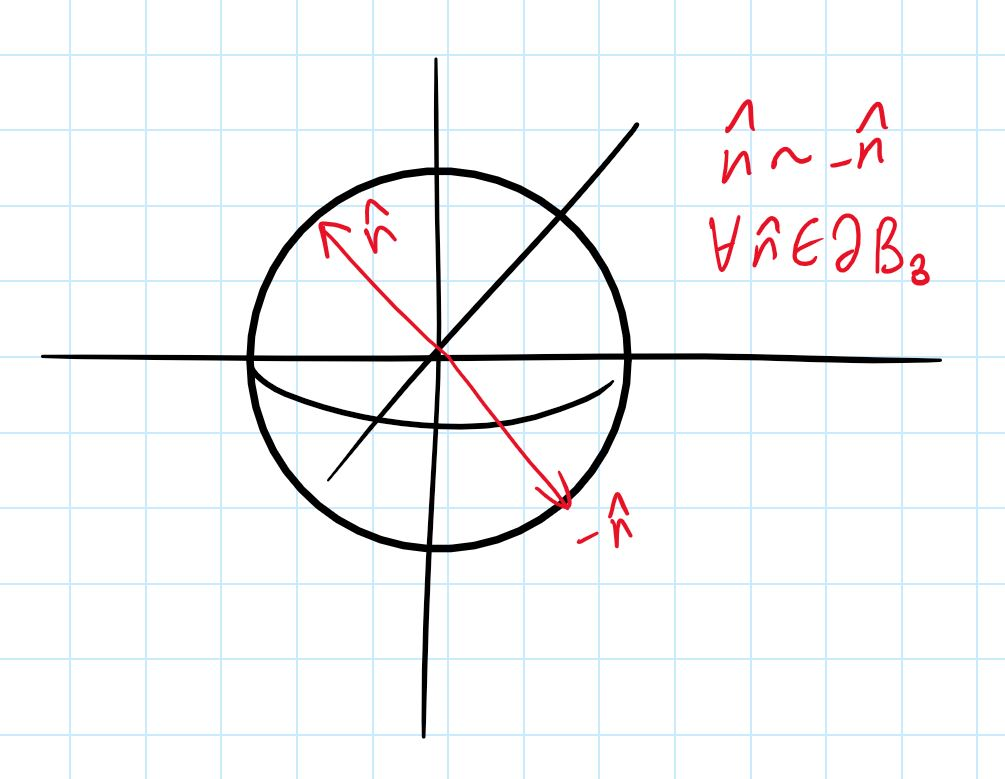
\includegraphics[scale=0.7]{2018/10/20181009_img1}
\caption{The group manifold $M(SO(3))$ is isomorphic to the 3-ball $B^3$ with antipodal points on the boundary identified, $\vec{w} \sim -\vec{w} \forall \vec{w} \in \p B_3$.}
\end{figure}

\begin{defn}
A \term{compact} set is any bounded, closed set in $\RR^n$ with $n\geq 0$. For instance, the $2$-sphere $S^2$ is clearly bounded in $\RR^3$. But the hyperboloid $H^2$ (embedded in $\RR^3$ as $x^2+y^2-z^2 =r^2$) is not bounded, since for any distance $r_0$ one can construct a point $\vec{x}$ on $H^2$ which has $|\vec{x}|>r_0$.
\end{defn}

Let us note some properties of the group manifold $M(SO(3))$. It is compact and connected, but it is not simply connected.
\begin{defn}
A space is \term{simply connected} if all loops on the space are contractible (in the language of algebraic topology, its fundamental group $\pi_1$ is trivial).
\end{defn}
A bit of intuition for why $M(SO(3))$ is topologically non-trivial: draw a path to the boundary, come out on the antipodal side, and go back to the origin. As it turns out, this is different from $S^1$ or the torus $T^2$: whereas these have the full $\ZZ$ as (part of) their fundamental groups ($T^2$ is simply $S^1\times S^1$), if we go around twice in $SO(3)$ we find that this new loop is actually a trivial loop (see Fig. \ref{z2inso3}). Therefore the fundamental group of $SO(3)$ is not infinite but the cyclic group $\ZZ_2$ (i.e. the set $\set{0,1}$ under the group operation $+\mod 2$).

\begin{figure}\label{z2inso3}
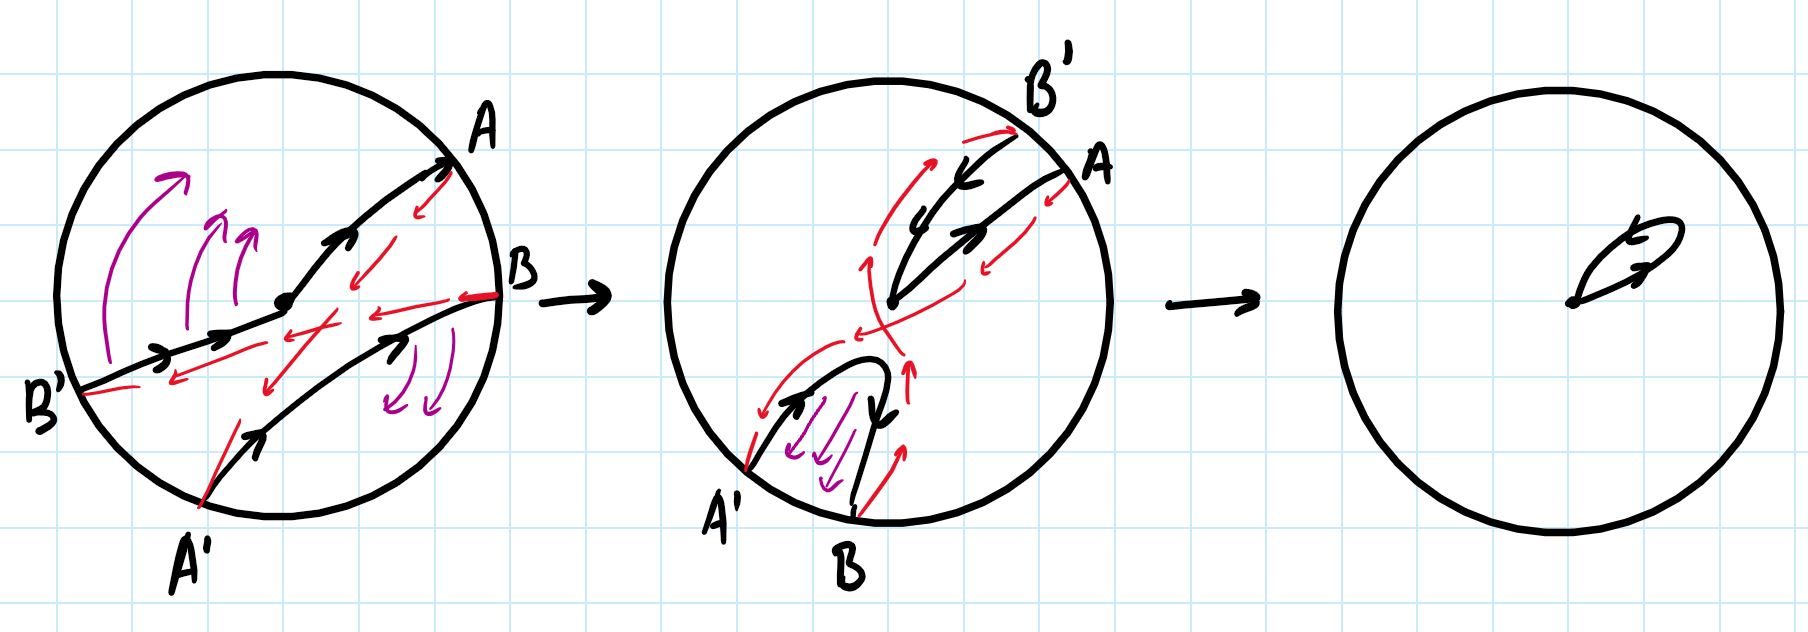
\includegraphics[scale=0.6]{2018/10/20181009_img2}
\caption{A sketch of why the loop which goes through the boundary $\p B_3$ twice is homotopic to (can be continuously deformed into) the trivial loop. For simplicity, consider a circular cross-section of $B_3$ and suppose the loop passes through the boundary at points $A$ ($\sim A'$) and $B$ ($\sim B'$). As we continuously move the point $B$ to $A'$, $B'$ must also move towards $A$, as we see in the second image. We then pull the bit of loop from $A'$ to $B$ through the boundary and find that the resulting loop is trivial (sketch 3). Solid black lines indicate the actual loop path, red dashed arrows indicate the effect of identifying antipodal points, and purple arrows suggest the direction of loop deformation between each drawing.}
\end{figure}
	
\end{document}